% Note that the text in the [] brackets is the one that will
% appear in the table of contents, whilst the text in the {}
% brackets will appear in the main thesis.

%% CHAPTER HEADER /////////////////////////////////////////////////////////////////////////////////////
\chapter[The Time-Domain \acs{sem} Formulation]{The Time-Domain Spectral Element Method Formulation}
\label{ch:sem}
%% CHAPTER INTRODUCTION ///////////////////////////////////////////////////////////////////////////////
The comprehensive formulation of the \ac{sem} based numerical model is presented in this chapter.
It includes shape function definition, numerical integration in the scheme of \ac{gll}, determination of the structural matrices for solid and first-order shear deformation theory elements and electromechanical coupling for the \acp{pzt}.
The non-matching interface was introduced with the novel approach based on the element shape functions.
All this is to implement the \ac{sem} for the honeycomb structure with the \ac{fcgm}, which is not found in the literature before.

%% INCLUDE SECTIONS ///////////////////////////////////////////////////////////////////////////////////
%% SECTION HEADER /////////////////////////////////////////////////////////////////////////////////////
\section{High order polynomial interpolation and the \acl{gll} integration scheme}
\label{sec:sem}

%% SECTION CONTENT ////////////////////////////////////////////////////////////////////////////////////

The \ac{sem} is similar to the \ac{fem}.
The similarity of both methods lies in the fact that considered domain is divided into non-overlapping finite elements, and external forces and arbitrary boundary conditions are imposed in the particular nodes.
The main difference between those methods is a selection of the shape function \( N=N(\xi )\), pictured in Figure~\ref{fig:shape}, which is interpolated by a Lagrange polynomial that passes through the element nodes.
The nodes are localised on the endpoint of an interval, \(\xi\in[-1,1]\), and the roots of the first derivative of Legendre polynomial \(\mathcal{P}\) of degree \(p\):
\begin{eqnarray}
	(1-\xi^2)\mathcal{P}'_{p}(\xi)=0.
	\label{eq:nodes}
	\nomtypeD[x]{\( \xi, \eta, \zeta \)}{Local coordinates}{}
	\nomtypeD[w]{\(w\)}{Weighting factor}{}
\end{eqnarray}
The approximation of an integral over the elements is achieved according to the \ac{gll} rule at points coinciding with the element nodes. The integration weights \(w=w(\xi)\) equal
\begin{eqnarray}
	{w(\xi)} = \frac{2}{p(p+1)(\mathcal{P}_{p}(\xi))^2}.
	\label{eq:weight}
\end{eqnarray}

The shape functions and the weights for \ac{2d} or \ac{3d} elements are obtained by the Kronecker product of vectors of individual axes, denoted by \(\otimes\) as follows:
\begin{eqnarray}
	\begin{array}{rcl}
	N(\xi,\eta) & = & N(\xi)\otimes N(\eta),\\
	N(\xi,\eta,\zeta) & = & N(\xi)\otimes N(\eta)\otimes N(\zeta),
	\end{array}
\label{eq:shape_functions}
\nomtypeD[N]{$N$}{Shape function}{}
\end{eqnarray}
\begin{eqnarray}
	\begin{array}{rcl}
	w(\xi,\eta) & = & w(\xi)\otimes w(\eta),\\
	w(\xi,\eta,\zeta) & = & w(\xi)\otimes w(\eta)\otimes w(\zeta).
	\end{array}
	\label{eq:weights}
\end{eqnarray}
\begin{figure}[H]
	\begin{center}
		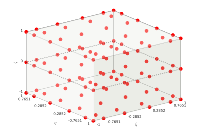
\includegraphics[width=0.95\textwidth]{Chapter_4/shape_function}
	\end{center}
	\caption{Shape functions based on fifth-order polynomial interpolation}
	\label{fig:shape}
\end{figure}

The derivation of the equation of motion is given in \cite{ostachowicz2011guided}, and it is defined as
\begin{eqnarray}
	\label{eq:motion}
	\textbf{M} \ddot{\textbf{d}} + \textbf{D} \dot{\textbf{d}} + \textbf{K} \textbf{d} = \textbf{f}_{ext},
	\nomtypeR[M]{$\textbf{M}$}{Mass matrix}{}{\unit{\kg}}%
	\nomtypeR[D]{$\textbf{D}$}{Damping matrix}{}{\unit[per-mode = symbol]{\newton\second \per \meter}}%
	\nomtypeR[K]{$\textbf{K}$}{Stiffness matrix}{}{\unit[per-mode = symbol]{\newton\per\metre}}%
	\nomtypeR[force_ext]{$\textbf{f}_{ext}$}{External force vector}{}{\unit{\newton}}%
	\nomtypeR[d]{$\textbf{d}$}{Displacements vector}{}{\unit{\meter}}%
\end{eqnarray}
where \textbf{d} is the displacements vector; \textbf{M}, \textbf{D} and \textbf{K} are the structural mass, damping and stiffness matrices, respectively; \textbf{F}$_{ext}$ is the external forces vector; \((\dot{\ })=\frac{\partial}{\partial t}\).
The construction of the structural matrices is similar to the classical approach in \ac{fem}.

The most significant advantage of this method is the fast convergence of the equation of motion.
It is achieved for six nodes per wavelength, while at least fifteen nodes are needed in the case of linear elements in classic \ac{fem}~\cite{wee2017simulating}.
In addition, the mass matrix is diagonal when using the \ac{gll} approach and solid elements or elements based on first-order shear deformation theory.

%% SECTION HEADER /////////////////////////////////////////////////////////////////////////////////////
\section{2D Spectral Modelling}
\label{sec:2Dmodel}

%% SECTION CONTENT ////////////////////////////////////////////////////////////////////////////////////

According to the first-order shear deformation theory~\cite{reissner1945effect, mindlin1951influence}, the displacement field is expressed as:
\begin{eqnarray}
	\left \{ \begin{array}{c}
		\textbf{u}^e(\xi,\eta) \\
		\textbf{v}^e(\xi,\eta) \\
		\textbf{w}^e(\xi,\eta)
	\end{array} \right\} = 
	\left \{ \begin{array}{c}
		\textbf{u}_0^e(\xi,\eta) + z\boldsymbol{\varphi}_x^e(\xi,\eta)\\
		\textbf{v}_0^e(\xi,\eta) + z\boldsymbol{\varphi}_y^e(\xi,\eta)\\
		\textbf{w}_0^e(\xi,\eta) \\
	\end{array} \right\},
\end{eqnarray}
where \(\textbf{u}_0^e\), \(\textbf{v}_0^e\) and \(\textbf{w}_0^e\) are nodal displacements, \(\boldsymbol{\varphi}_x^e\), \(\boldsymbol{\varphi}_y^e\) are the rotations of the normal to the mid-plane with respect to the axes \textit{x} and \textit{y}, respectively.
\begin{eqnarray}
	\left \{\begin{array}{c}
		\textbf{u}_0^e(\xi,\eta) \\
		\textbf{v}_0^e(\xi,\eta) \\
		\textbf{w}_0^e(\xi,\eta) \\
		\boldsymbol{\varphi}_x^e(\xi,\eta) \\
		\boldsymbol{\varphi}_y^e(\xi,\eta)
	\end{array} \right\}
	= \textbf{N}^e(\xi,\eta)\widehat{\textbf{d}}^e
	= \sum_{n=1}^q\sum_{m=1}^p\textbf{N}_m^e(\xi)\textbf{N}_n^e(\eta)
	\left \{ \begin{array}{c}
		\widehat{\textbf{u}}_0^e \\
		\widehat{\textbf{v}}_0^e \\
		\widehat{\textbf{w}}_0^e \\
		\widehat{\boldsymbol{\varphi}}_x^e \\
		\widehat{\boldsymbol{\varphi}}_y^e
	\end{array} \right \}.
\end{eqnarray}

The nodal bending strain--displacement relations are given in the form:
\begin{eqnarray}
	\boldsymbol{\epsilon}_b^e =
	\textbf{B}_b^e\widehat{\textbf{d}}^e = 
	\left [
	\begin{array}{ccccc}
		\frac{\partial N^e}{\partial x} & 0 & 0 & 0 & 0\\
		0 & \frac{\partial N^e}{\partial y} & 0 & 0 & 0\\
		\frac{\partial N^e}{\partial y} & \frac{\partial N^e}{\partial x} & 0 & 0 & 0\\
		0 & 0 & 0 & -\frac{\partial N^e}{\partial x} & 0\\
		0 & 0 & 0 & 0 & -\frac{\partial N^e}{\partial y}\\
		0 & 0 & 0 & -\frac{\partial N^e}{\partial y} & -\frac{\partial N^e}{\partial x}
	\end{array} \right]
	\left \{ \begin{array}{c}
		\widehat{\textbf{u}}_0^e \\
		\widehat{\textbf{v}}_0^e \\
		\widehat{\textbf{w}}_0^e \\
		\widehat{\boldsymbol{\varphi}}_x^e \\
		\widehat{\boldsymbol{\varphi}}_y^e
	\end{array} \right\}.
\end{eqnarray}

The nodal shear strain--displacement relations are given in the form:
\begin{eqnarray}
	\boldsymbol{\epsilon}_s^e =
	\textbf{B}_s^e\widehat{\textbf{d}}^e = 
	\left [
	\begin{array}{ccccc}
		0 & 0 & \frac{\partial N^e}{\partial y} & -1 & 0\\
		0 & 0 & \frac{\partial N^e}{\partial y} & 0 & -1
	\end{array} \right]
	\left \{ \begin{array}{c}
		\widehat{\textbf{u}}_0^e \\
		\widehat{\textbf{v}}_0^e \\
		\widehat{\textbf{w}}_0^e \\
		\boldsymbol{\varphi}_x^e \\
		\boldsymbol{\varphi}_y^e
	\end{array} \right\}.
\end{eqnarray}
%% SECTION HEADER /////////////////////////////////////////////////////////////////////////////////////
\section{3D Spectral Modelling}
\label{sec:3Dmodel}

%% SECTION CONTENT ////////////////////////////////////////////////////////////////////////////////////
The displacement vector of the \ac{3d} element is composed of three translational displacements defined as:
\begin{eqnarray}
	\left \{ \begin{array}{c}
		\textbf{u}^e(\xi,\eta,\zeta) \\
		\textbf{v}^e(\xi,\eta,\zeta) \\
		\textbf{w}^e(\xi,\eta,\zeta)
	\end{array} \right\}
	= \textbf{N}^e(\xi,\eta, \zeta)\widehat{\textbf{d}}^e
	= \sum_{l=1}^r\sum_{n=1}^q\sum_{m=1}^p\textbf{N}_m^e(\xi)\textbf{N}_n^e(\eta)\textbf{N}_l^e(\zeta)
	\left \{ \begin{array}{c}
		\widehat{\textbf{u}}^e(\xi_m,\eta_n,\zeta_l) \\
		\widehat{\textbf{v}}^e(\xi_m,\eta_n,\zeta_l) \\
		\widehat{\textbf{w}}^e(\xi_m,\eta_n,\zeta_l)
	\end{array} \right\},
	\label{eq:3D_displ}
\end{eqnarray}
where \(\widehat{\textbf{u}}^e\), \(\widehat{\textbf{v}}^e\) and 
\(\widehat{\textbf{w}}^e\) are displacements of the element nodes in \(\xi,\eta\) and \(\zeta\) direction.

The nodal strain--displacement relations are given as \cite{kudela20093d}:
\begin{eqnarray}
	\boldsymbol{\epsilon}^e=\textbf{B}_{d}^e\widehat{\textbf{d}}^e=
	\left [
	\begin{array}{ccc}
		\frac{\partial N^e}{\partial x} & 0 & 0\\
		0 & \frac{\partial N^e}{\partial y} & 0\\
		0 & 0 & \frac{\partial N^e}{\partial z}\\
		0 & \frac{\partial N^e}{\partial z} & \frac{\partial N^e}{\partial y}\\
		\frac{\partial N^e}{\partial z} & 0 & \frac{\partial N^e}{\partial x}\\
		\frac{\partial N^e}{\partial y} & \frac{\partial N^e}{\partial x} & 0
	\end{array} \right]
	\left \{ \begin{array}{c}
		\widehat{\textbf{u}}^e \\
		\widehat{\textbf{v}}^e \\
		\widehat{\textbf{w}}^e
	\end{array} \right\}.
\end{eqnarray}
The formulae of the structural matrices for 3D elements are:
\begin{eqnarray}
	\textbf{M}_{dd}^e & = & \int_{V_e}\textbf{N}^T\rho \textbf{N} \diff V_e,\\
	\textbf{K}_{dd}^e & = & \int_{V_e}{\textbf{B}_d^e}^T\textbf{C}\textbf{B}_d^e \diff V_e,
\end{eqnarray}
where \textbf{C} is the stiffness tensor, \(\rho\) is mass density, and \(V_e\) is the element volume.
%% SECTION HEADER /////////////////////////////////////////////////////////////////////////////////////
\section{\Acs{pzt} modelling}
\label{sec:PZTmodel}

%% SECTION CONTENT ////////////////////////////////////////////////////////////////////////////////////
The electromechanical coupling is governed by the linear constitutive equation of piezoelectric material according to~\cite{giurgiutiu2009micromechatronics, rekatsinas2017cubic}, and this is defined as:
\begin{eqnarray}
	\left [ 
	\begin {array}{c}
	\boldsymbol{\sigma}\\
	\widetilde{\textbf{D}}
\end{array}\right ]=
\left [ 
\begin{array}{cc}
	\textbf{c}^E & -\textbf{e}^{\mathrm{T}} \\
	\textbf{e} & \epsilon^S 
\end{array} \right ]
\left[ 
\begin{array}{c}
	\boldsymbol{\varepsilon}\\
	\widetilde{\textbf{E}} 
\end{array} \right ],
\label{eq:elecmechcoupling}
\end{eqnarray}
\nomtypeR[Ep]{$\widetilde{\textbf{E}} $}{Electric field}{\(-\textbf{B}\,\boldsymbol{\phi}\)}{\unit[per-mode=symbol]{\newton\per\coulomb}}%
\nomtypeR[Dp]{$\widetilde{\textbf{D}} $}{Electric charge density displacement}{-}{\unit[per-mode=symbol]{\coulomb\per\square\metre}}%
\nomtypeG[phip]{$\boldsymbol{\phi}$}{Electric potential vector}{-}{\unit{\volt}}%
\nomtypeG[sigma]{$\boldsymbol{\sigma}$}{Stress tensor}{\(\textbf{c}\,\boldsymbol{\varepsilon}\)}{\unit{\pascal}}%
where \(\boldsymbol{\sigma}\) is the stress components, \(\textbf{c}^E\) is the stiffness coefficient matrix measured at zero electric field, \textbf{e} is the piezoelectric coupling tensor, \(\boldsymbol{\epsilon}^S\) is the electric permittivity measured at zero strain, and \(\widetilde{\textbf{E}}\) and \(\widetilde{\textbf{D}}\) are the electric field and electric charge density displacement.
The electric field of the element is defined as:
\begin{eqnarray}
\widetilde{\textbf{E}}^e=-\textbf{B}_\phi^e \widehat{\boldsymbol{\phi}}^e = \left[ \begin{array}{c}
	\frac{\partial N^e}{\partial \xi}\\
	\frac{\partial N^e}{\partial \eta}\\
	\frac{\partial N^e}{\partial \zeta}
\end{array} \right] \widehat{\boldsymbol{\phi}}^e,
\end{eqnarray}
where \(\widehat{\boldsymbol{\phi}}^e\) is a nodal voltage of the transducer. The \ac{sem} formulation of the governing equation (\ref{eq:elecmechcoupling}) is defined as:
\begin{eqnarray}
	\left [\begin{array}{cc}
		\textbf{M}_{dd} & \textbf{0}\\
		\textbf{0} & \textbf{0}
	\end{array}\right]
	\left \{\begin{array}{c}
		\widehat{\ddot{\textbf{d}}} \\
		\textbf{0}
	\end{array}\right \} +
	\left [\begin{array}{cc}
		\textbf{K}_{dd} & \textbf{K}_{d \phi}\\
		\textbf{K}_{d \phi}^{\mathrm{T}} & \textbf{K}_{\phi \phi}
	\end{array}\right]
	\left \{\begin{array}{c}
		\widehat{\textbf{d}} \\
		\widehat{\boldsymbol{\phi}}
	\end{array}\right \}  = 
	\left \{\begin{array}{c}
		\textbf{0}\\
		\widehat{\textbf{Q}}
	\end{array}\right \},
	\label{eq:pzt_sem}
\end{eqnarray}
\nomtypeR[Q]{$\textbf{Q}$}{Charge vector}{-}{\unit{\coulomb}}%
where \(\widehat{\textbf{Q}}\) is the nodal charge vector.
The mass and stiffness matrices are defined according to \ac{3d} model from section \ref{sec:3Dmodel}.
The piezoelectric coupling matrix \(\textbf{K}_{\phi \phi}^e\) and the dielectric permittivity matrix \(\textbf{K}_{d \phi}^e\) are defined as:
\begin{eqnarray}
	\textbf{K}_{d\phi}^e & = & \int_{V_e}{\textbf{B}_d^e}^{\mathrm{T}}\textbf{e}^{\mathrm{T}} \textbf{B}_{\phi}^e \diff V_e,\\
	\textbf{K}_{\phi \phi}^e & = & -\int_{V_e}{\textbf{B}_{\phi}^e}^{\mathrm{T}} 
	{\textbf{\(\epsilon\)}^S}^{\mathrm{T}} \textbf{B}_{\phi}^e \diff V_e.
\end{eqnarray}

If a vector \(\textbf{b}\) contains list of consecutive boundary nodes (corresponding to electrodes) and a vector \(\textbf{a}\) contains lists of consecutive active nodes (remaining nodes) of the \ac{pzt}, the electrical potential vector and the charge vector can be rewritten as:
\begin{eqnarray}
	\widehat{\boldsymbol{\phi}} & = & \left \{\begin{array}{cc}
		\widehat{\boldsymbol{\phi}}(\textbf{b}) &
		\widehat{\boldsymbol{\phi}}(\textbf{a})
	\end{array}\right \}^{\mathrm{T}},\\
	\widehat{\textbf{Q}} & = & \left \{\begin{array}{cc}
		\widehat{\textbf{Q}}(\textbf{b}) & \textbf{0}
	\end{array}\right \}^{\mathrm{T}}.
	\label{eq:phi_Q}
\end{eqnarray}
Then, piezoelectric part of Eq.~(\ref{eq:pzt_sem}) is expressed as:
\begin{eqnarray}
	\begin{split}
		\left [\begin{array}{cc}
			\textbf{K}_{d \phi}(:,\textbf{b}) &
			\textbf{K}_{d \phi}(:,\textbf{a})
		\end{array}\right]^{\mathrm{T}}
		\widehat{\textbf{d}} & +
		\left [\begin{array}{cc}
			\textbf{K}_{\phi \phi}(\textbf{b},\textbf{b}) & \textbf{K}_{\phi 		\phi}(\textbf{b},\textbf{a})\\
			\textbf{K}_{\phi \phi}(\textbf{a},\textbf{b}) & \textbf{K}_{\phi \phi}(\textbf{a},\textbf{a})
		\end{array}\right]
		\left \{\begin{array}{c}
			\widehat{\boldsymbol{\phi}}(\textbf{b}) \\
			\widehat{\boldsymbol{\phi}}(\textbf{a})
		\end{array}\right \}\\ 
		& = \left \{\begin{array}{c}
			\widehat{\textbf{Q}}(\textbf{b}) \\
			\textbf{0}
		\end{array}\right \},
	\end{split}
	\label{eq:pztboundary}
\end{eqnarray}
where the notation \(\textbf{K}(\textbf{r},\textbf{c})\) uses vectors \(\textbf{r}\) and \(\textbf{c}\) to extract rows and columns from the matrix \(\textbf{K}\), respectively, and \((:)\) means all rows or columns of \(\textbf{K}\).
The electrical potential of the free nodes can be extracted from Eq.~(\ref{eq:pztboundary}):
\begin{eqnarray}
	\widehat{\boldsymbol{\phi}}(\textbf{a}) = -\textbf{K}_{\phi\phi}^{-1}(\textbf{a},\textbf{a})\left[\textbf{K}_{\phi d}(\textbf{a},:) \widehat{\textbf{d}} + \textbf{K}_{\phi\phi}(\textbf{a},\textbf{b})\widehat{\boldsymbol{\phi}}(\textbf{b}) \right].
	\label{eq:freePotetial}
\end{eqnarray}
If the \ac{pzt} acts as an actuator, the electrical potential of the electrode nodes has the values of the applied signal.
As one of the electrodes is grounded, the potential is zero.
Therefore, the potential vector can be written as:
\begin{eqnarray}
	\widehat{\boldsymbol{\phi}}(\textbf{b}) = \left \{\begin{array}{cc}
		\widehat{\boldsymbol{\phi}}(\textbf{b}_v) &
		\widehat{\boldsymbol{\phi}}(\textbf{b}_g)
	\end{array}\right \}^{\mathrm{T}}=\left \{\begin{array}{cc}
	\textbf{V}(t) & \textbf{0}
	\end{array}\right \}^{\mathrm{T}},
	\label{eq:phi_V}
\end{eqnarray}
where \(\textbf{b}_v\) is a list of nodes of the applied electrode and \(\textbf{b}_g\) is a list of nodes of the grounded electrode.
Substituting Eq. (\ref{eq:phi_V}) into Eq. (\ref{eq:freePotetial}) and Eq. (\ref{eq:pztboundary}), induced stiffness of the actuator is obtained:
\begin{eqnarray}
	\textbf{K}_{a}=-\textbf{K}_{d\phi}(:,\textbf{a})\,\textbf{K}_{\phi \phi}^{-1}(\textbf{a},\textbf{a})\,\textbf{K}_{\phi \phi} (\textbf{a},\textbf{b}).
\end{eqnarray}
Hence, the equivalent mechanical force vector of the applied voltage of the piezoelectric actuator equals:
\begin{eqnarray}
	\widehat{\textbf{f}}_{a}=-\textbf{K}_{a}\,\widehat{\boldsymbol{\phi}}(\textbf{b}).
	\label{eq:f_act}
\end{eqnarray}
\nomtypeR[force_act]{$\textbf{f}_{a}$}{Actuator equivalent force vector}{\(-\textbf{K}_a\,\boldsymbol{\phi}(b)\)}{\unit{\newton}}%
In the case of the open circuit sensor one electrode is grounded so the electric potential of the free nodes becomes as:
\begin{eqnarray}
	\widehat{\boldsymbol{\phi}}(\textbf{a}) = -\textbf{K}_{\phi\phi}^{-1}(\textbf{a},\textbf{a})\,\textbf{K}_{\phi d}(\textbf{a},:)\,\widehat{\textbf{d}}.
	\label{eq:sensorPotetial}
\end{eqnarray}
The induced stiffness of the sensor can be written as:
\begin{eqnarray} \textbf{K}_s=\textbf{K}_{d \phi}(:,\textbf{a})\,\textbf{K}_{\phi \phi}^{-1} (\textbf{a},\textbf{a})\,\textbf{K}_{\phi d}(\textbf{a},:).
\end{eqnarray}
To obtain the sensor response, the nodal electric potential must be integrated over the electrode surface as follow:
\begin{eqnarray}
	\boldsymbol{\phi}(t) = \int_{\Omega_s}\widehat{\phi} \diff\Omega_s.
	\label{eq:sensorResponse}
\end{eqnarray}
%% SECTION HEADER /////////////////////////////////////////////////////////////////////////////////////
\section{Structural damping}
\label{sec:damping}

%% SECTION CONTENT ////////////////////////////////////////////////////////////////////////////////////
Propagating waves in the structure attenuate due to many factors, including geometric spreading, material damping, and dissipation into the adjacent domain.
This study adopted the Rayleigh damping model for the \ac{cfrp} skin and adhesive layer, while the damping for the aluminium core and the \ac{pzt} was neglected.
According to \cite{wandowski2017guided}, the Rayleigh damping model is defined as
\begin{eqnarray}
	\textbf{D}_{dd}^e = \alpha_M \textbf{M}_{dd}^e + \beta_K \textbf{K}_{dd}^e,
	\label{eq:damping}
	\nomtypeD[alpha]{$\alpha_M$}{Mass-proportionality damping coefficient}{}%
	\nomtypeD[beta]{$\beta_K$}{Stiffness-proportionality damping coefficient}{}%
\end{eqnarray}
where \(\alpha_M\) and \(\beta_K\) are the mass- and stiffness- proportionality coefficients.
In the presented model, \(\beta_K\) was assumed to be zero to ensure that matrix \(\textbf{D}_{dd}\) remains diagonal \cite{schulte2011simulation, wandowski2017guided}.
This assumption gives a good approximation when considering a single mode and a specific frequency. 
Ramadas showed slight differences in Lamb wave attenuation by analysing three models, i.e. mass-, stiffness-proportional and the sum of both \cite{ramadas2011modelling}.
However, due to the diagonal damping matrix, the mass-proportional model is computationally more efficient than the other models.
%% SECTION HEADER /////////////////////////////////////////////////////////////////////////////////////
\section{Displacements coupling at the interface of substructures}
\label{sec:interface}

%% SECTION CONTENT ////////////////////////////////////////////////////////////////////////////////////
The proposed model of the sandwich panel consisted of \ac{2d} and \ac{3d} elements.
In the combination of such elements, there are no common nodes because the nodes of the shell element are localised on the mid-plane of the component.
I realised the connection of both elements in a paper regarding the research on the effect of the glue thickness between the \ac{pzt} and the host plate on the propagation of elastic waves in a composite plate \cite{fiborek20192d}.
Connection was made possible by incorporating interface elements between both components.
The interface was implemented based on Lagrange multipliers, which are interpreted as forces imposed to determine the appropriate displacements of the nodes. My approach was similar to the interface for two shell elements proposed by Ashawin et al. \cite{ashwin2014formulation}.
To avoid creating coincided meshes for all components of \ac{hsc}, a non-matching interface should be used.
For this purpose, I proposed a novel approach for Lagrange multipliers-based interface, which creates a coupling matrix by the spectral elements shape function.
The non-matching interface was incorporated in the simulations of \ac{gw} registered by the \ac{fbg} optical sensor \cite{fiborek2022spectral}.
This paper is an original work regarding modelling such a sensor by the \ac{sem}.

\begin{figure}[!htb]
	\begin{center}
		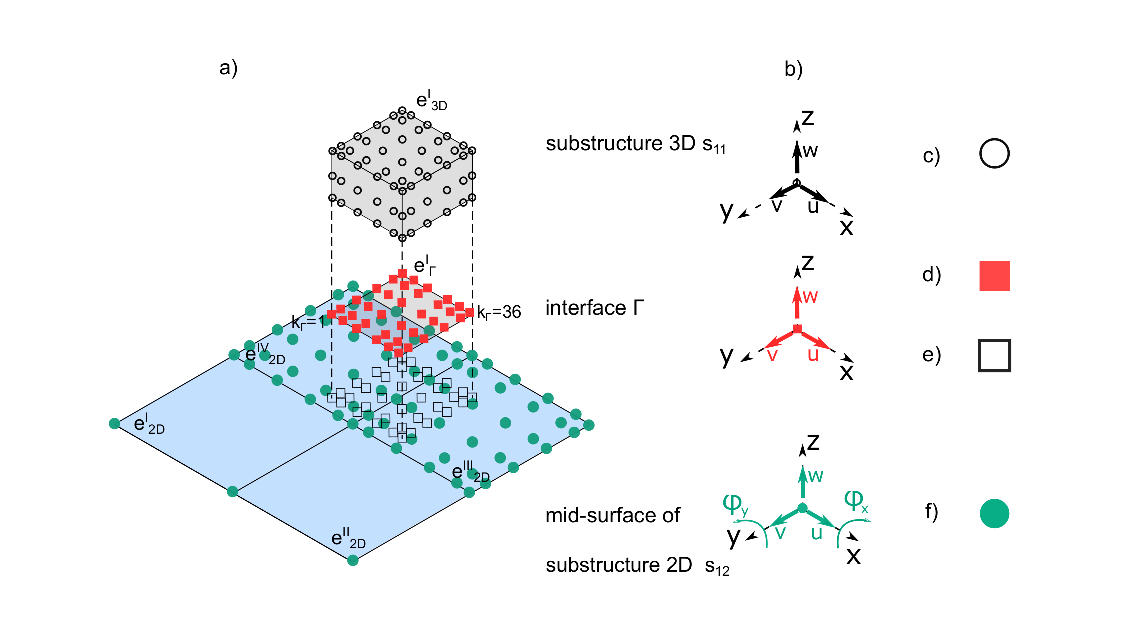
\includegraphics[width=1\textwidth]{Chapter_4/interface_2D3D}
	\end{center}
	\caption{Non-matching interface setup: (\textbf{a}) interface coupling, (\textbf{b}) the interface and the substructures degrees-of-freedom}
	\label{fig:interface}
\end{figure}
The non-matching interface between \ac{2d} and \ac{3d} elements is presented in Figure~\ref{fig:interface}.
The coupling of two domains imposes zero displacements relative to each other.
It can be expressed as
\begin{eqnarray}
	\left\{\begin{array}{c}
		\textbf{u}\\
		\textbf{v}\\
		\textbf{w}
	\end{array}\right\}_{s_{i1}}^{\Gamma^i}-
	\left\{\begin{array}{c}
		\textbf{u}\\
		\textbf{v}\\
		\textbf{w}
	\end{array}\right\}_{s_{i2}}^{\Gamma^i}=
	\left\{\begin{array}{c}
		\textbf{0}\\
		\textbf{0}\\
		\textbf{0}
	\end{array}\right\},
	\label{eq:coupling}
	\nomtypeD[Gamma]{$\Gamma$}{Interface}{}
\end{eqnarray}
where \(s_{i1}\) and \(s_{i2}\) are components connected by the interface \(\Gamma^i\).
For the whole structure, the Eq.~(\ref{eq:coupling}) can be written in the matrix form
\begin{eqnarray}
	\textbf{G}\textbf{d}=\textbf{0},
	\label{eq:cond_disp}
	\nomtypeD[G]{$\textbf{G}$}{Interface coupling matrix}{}
\end{eqnarray}
where \textbf{G} is the coupling matrix which contains the equations to interpolate the substructures displacements at the interfaces, and \(\textbf{d}\) is a global displacement field for \(nS\) number of substructures, composed as
\begin{eqnarray}
	\textbf{d} = \left\{\begin{array}{cccc}
		\textbf{d}_1, & \textbf{d}_2, &\ldots, & \textbf{d}_{nS}
	\end{array}\right\}^T.
	\label{eq:displacements}
\end{eqnarray}

\begin{algorithm}[!tbh]
	\SetAlgoLined
	\For{i = 1 \KwTo 2}{
		create \(n^{\Gamma}\times n^{s_i}\) null matrix 
		\(\mathbf{G}_i\),\\
		\For{j = 1 \KwTo \(n^{\Gamma}\)} {
			find \(ownerElement^j_i\) in the structure \(s_i\)
			containing interface node \(j\) with global coordinates vector: 
			\(X_p=(x^j_p,y^j_p)\)\;
			assign vector \(X_e=(x_e,y_e)\) of coordinates of all nodes in 
			\(ownerElement^j_i\)\;
			assign initial coordinates 
			\(X_{\kappa}=(x^j_{\kappa},y^j_{\kappa})\) to the nearest node in
			\(ownerElement^j_i\) to node \(j\)\;
			transform global coordinates \(X_{\kappa}\) to a local coordinate system \(\xi_{\kappa}=\xi(X_{\kappa}),\  
			\eta_{\kappa}=\eta(X_{\kappa})\)\;
			\While{\(\left|X_p-X_{\kappa}\right|>\mathrm{tol}\)}{
				\(\xi_{\kappa+1}=\xi_{\kappa}+(\mathcal{J}_{\kappa})^{1,1}_{\mathrm{inv}}(x^j_p-x_{\kappa}^j)
				+(\mathcal{J}_{\kappa})^{1,2}_{\mathrm{inv}}(y^j_p-y_{\kappa}^j)\)\,
				\(\eta_{\kappa+1}=\eta_{\kappa}+(\mathcal{J}_{\kappa})^{2,1}_{\mathrm{inv}}(x^j_p-x_{\kappa}^j)
				+(\mathcal{J}_{\kappa})^{2,2}_{\mathrm{inv}}(y^j_p-y_{\kappa}^j)\)\,
				\(X_{\kappa}=N_{\kappa+1}X_e\)\,
			}
			\(\mathbf{G}_i(j,n^{X_e})=N_{\kappa+1}\)\;
		}
		\uIf{\(s_i\) \(\mathrm{is\ 3D}\)} {
			\(\mathbf{G}_i=\left[\begin{array}{ccc}
				\mathbf{G}_i & \mathbf{0} & \mathbf{0}\\
				\mathbf{0} & \mathbf{G}_i & \mathbf{0}\\
				\mathbf{0} & \mathbf{0} & \mathbf{G}_i
			\end{array} \right]
			\)\;
		}
		\ElseIf{\(s_i\) \(\mathrm{is\ 2D}\)} {
			\(\mathbf{G}_i=\left[\begin{array}{ccccc}
				\mathbf{G}_i & \mathbf{0} & \mathbf{0} & 
				\frac{h_i}{2}\mathbf{G}_i & \mathbf{0}\\
				\mathbf{0} & \mathbf{G}_i & \mathbf{0} & \mathbf{0} & 
				\frac{h_i}{2}\mathbf{G}_i\\
				\mathbf{0} & \mathbf{0} & \mathbf{G}_i & \mathbf{0} & 
				\mathbf{0}
			\end{array} \right]\)\;
		}
	}
	\KwResult{coupling matrix \(\mathbf{G}=\left[\begin{array}{cc}
			\mathbf{G}_1 & \mathbf{G}_2
		\end{array} \right]\)}
	where \(s_i\) is one of the coupled structures,\;
	\(n^{\Gamma}\) and \(n^{s_i}\) are node numbers of the interface and node numbers of the structure \(s_i\), respectively \; \(\left(\mathcal{J}_{\kappa}\right)_{\mathrm{inv}}\) is the inverse Jacobian matrix evaluated at \((\xi_{\kappa},\eta_{\kappa})\)\;
	\(N_{\kappa+1}\) is the shape function evaluated at \((\xi_{\kappa+1},\eta_{\kappa+1})\)\;
	\(n^{X_e}\) is the vector of global order numbers of all nodes in the \(ownerElement^j_i\)\;
	\(h_i\) is a thickness of the structure \(s_i\) and tol is a termination criterion for iterations.
	\caption{Interface coupling matrix formulation}
	\label{alg:G_matrix}
	\nomtypeD[Jacobian]{$\mathcal{J}$}{Jacobian matrix}{}%
	\nomtypeD[nmn]{$n,m,n$}{Nodes numbers}{}%
	\nomtypeR[Xp]{$X_p$}{Coordinates vector of the interface point}{}{\unit{\metre}}%
	\nomtypeR[Xe]{$X_e$}{Coordinates vector of the element nodes}{}{\unit{\metre}}%
\end{algorithm}
General formulation of the matrix \textbf{G} is presented in Algorithm \ref{alg:G_matrix}.
The main task in this procedure was to calculate shape functions for each adjacent substructure at the points \(X_p=(x_p^k,y_p^k)\), which are projections of the interface nodes onto these substructures.
The shape function can be calculated after finding an owner element and local coordinates of the points.
Owner element is a spectral element in the domain of the substructure \(s_{ij}\) which contains interface node, for example, interface node \(k_\Gamma=36\) shown in~Figure~\ref{fig:interface}(\textbf{a}) is located in the element \(e^{I}_{3\mathrm{D}}\) and \(e^{III}_{2\mathrm{D}}\) for the substructures \(s_{11}\) and \(s_{12}\), respectively.
It can be found in two ways: using Matlab's built-in function \verb+inpolygon+ or more efficient procedure proposed by Silva et al. \cite{silva2009exact} which was used in the current implementation.
In this procedure, an initial approximation was first performed by rejecting all external points outside the rectangular region bounded by the points \(\mathrm{P_{min}}\) and \(\mathrm{P_{max}}\) as shown in Figure \ref{fig:b_b_test}(\textbf{a}).
If \(\mathrm{X_p}\) is inside the element, then the vectors \(\vec{V}_1\) and \(\vec{V}_2\) have the same direction.
\(\vec{V}_1\) and \(\vec{V}_2\) are defined as
\begin{eqnarray}
	\vec{V}_1 & = & \vec{v}_1\times \vec{v}_p,\\
	\vec{V}_2 & = & \vec{v}_p\times \vec{v}_2.
\label{eq:v_vectors}
\nomtypeD[vvv]{$\vec{v}_p,\,\vec{v}_1,\,\vec{v}_2$}{Cross-product test  vectors}{}%
\nomtypeD[V1]{$\vec{V_1}$}{First cross-product vector}{}%
\nomtypeD[V2]{$\vec{V_2}$}{Second cross-product vector}{}%
\end{eqnarray}
The vectors \(\vec{v}_p\), \(\vec{v_1}\) and \(\vec{v_2}\) are pictured in Figure \ref{fig:b_b_test}(\textbf{b}). \(\vec{V}_1\) and \(\vec{V}_2\) have the same direction if the inequality \(\vec{V}_1 \cdot \vec{V}_2 \geq0\) is satisfied for each element vertex.
Then, the transformation from global to local coordinates was realised by the iterative method presented in the work of Li et al.~\cite{li2014efficient} (see also \verb+while-loop+ in Algorithm~\ref{alg:G_matrix}).
\begin{figure}[!tbh]
	\begin{center}
		\includegraphics[width=0.95\textwidth]{Chapter_4/b_b_test}
	\end{center}
	\caption{Owner element for Xp interface node (\textbf{a}) boundary test, (\textbf{b}) cross-product test}
	\label{fig:b_b_test}
\end{figure}
As the cross product test is applicable only for elements with linear edges, in the case of boundaries approximated by second-order elements, this test was omitted.

The computational effectiveness of Algorithm~\ref{alg:G_matrix} can be easily improved if certain precautions are taken.
Firstly, the mesh of the interface has to be based on the mesh from one of the substructures \(s_{i}\), which may be referred to as a slave.
Shape functions evaluated at (\(\xi\), \(\eta\)) may take only zero and one values.
Moreover, the code was vectorised rather than using a for-loop form, provided that the required matrix of size \(4n^e\times n^{\Gamma}\), where \(n^e\) is the number of elements of the structure \(s_i\) elements, does not exceed the operating memory.
%% SECTION HEADER /////////////////////////////////////////////////////////////////////////////////////
\section{The time integration algorithm}
\label{sec:time}

%% SECTION CONTENT ////////////////////////////////////////////////////////////////////////////////////
The time integration algorithms for the wave propagation can be realised by the step-by-step methods, named Newmark family schemes \cite{newmark1959method}.
The schemes are in general form as
\begin{eqnarray}
	\label{eq:u_newmark}
	\textbf{d}_{t+\Delta t} & = & \textbf{d}_{t} +\Delta t \dot{\textbf{d}}_{t} + \left( 0.5 - \beta \right)\Delta t^2\ddot{\textbf{d}}_{t} + \beta \Delta t^2\ddot{\textbf{d}}_{t+\Delta t},\\
	\dot{\textbf{d}}_{t+\Delta t} & = & \dot{\textbf{d}}_{t} + \Delta t\left(1-\gamma\right)\ddot{\textbf{d}}_{t} + \gamma \Delta t\ddot{\textbf{d}}_{t+\Delta t},
\end{eqnarray}
\nomtypeG[Deltat]{$\Delta t$}{Time increment}{}{\unit{\second}}%
\nomtypeD[betagamma]{$\beta,\,\gamma$}{Time integration parameters}{}%
where \(\Delta t\) is the time increment, \(\textbf{d}_{t}\), and \(\textbf{d}_{t+\Delta t}\) are the displacement vectors in time t, and one step forward, respectively, and \(\beta\) and \(\gamma\) are the integration parameters.
The time discretisation for \(\beta = 0.25\) and \(\gamma = 0.5\), is second-order accurate and the algorithm is a stable, i.e., independent of the time step. It is called an implicit algorithm.
In the case of \(\beta = 0\) and \(\gamma = 0.5\) explicit algorithm is obtain and it is named the central difference method.
In this method for the solution convergence, a time step must be taken much smaller than the Nyquist-Shannon sampling theorem requires.

Considering piezoelectric coupling given by Eq.~(\ref{eq:elecmechcoupling}) and the displacement interface coupling represented by Eq.~(\ref{eq:cond_disp}) the global equation of motion is expressed as
\begin{eqnarray}
	\label{eq:motion_coupling}
	\textbf{M}_{dd}\,\widehat{\ddot{\textbf{d}}} +
	\textbf{D}_{dd}\,\widehat{\dot{\textbf{d}}} +
	\left [\begin{array}{ccc}
		\textbf{K}_{dd}&\textbf{K}_{d\phi}&\textbf{G}^T\\
		\textbf{K}_{d\phi}^T&\textbf{K}_{\phi \phi}&\textbf{0}\\
		\textbf{G}&\textbf{0}&\textbf{0}
	\end{array}\right]
	\left \{\begin{array}{c}
		\widehat{\textbf{d}}\\
		\widehat{\boldsymbol{\phi}}\\
		\widehat{\boldsymbol{\lambda}}
	\end{array}\right\} =
	\left \{\begin{array}{c}
		\widehat{\textbf{f}}_{ext} \\
		\widehat{\textbf{Q}}\\
		\textbf{0}
	\end{array}\right \},
\end{eqnarray}
\nomtypeD[lambda]{$\boldsymbol{\lambda}$}{Lagrange multipliers vector}{}%
where \(\widehat{\boldsymbol{\lambda}}\) is the nodal Lagrange multipliers vector.
Substituting Eq.~(\ref{eq:pztboundary}) and Eq.~(\ref{eq:freePotetial}) into Eq.~(\ref{eq:motion_coupling}), the equation of motion can be rearranged into the form
\begin{eqnarray}
	\textbf{M}_{dd}\,\widehat{\ddot{\textbf{d}}} + \textbf{D}_{dd} \,\widehat{\dot{\textbf{d}}} + (\textbf{K}_{dd}-\textbf{K}_{s}) \,\widehat{\textbf{d}}  = \widehat{\textbf{f}}_{ext} + \widehat{\textbf{f}}_{a} - \textbf{G}^{\mathrm{T}}\,\widehat{\boldsymbol{\lambda}}.
	\label{eq:motionD}
\end{eqnarray}
In the scheme of central difference method, the velocity and acceleration at a certain time \(t\) is given by
\begin{eqnarray}
	\label{eq:v}
	\widehat{\dot{\textbf{d}}}_{t} & = & \frac{\widehat{\textbf{d}}_{t+\Delta t} - \widehat{\textbf{d}}_{t-\Delta t}}{2\Delta t},\\
	\label{eq:a}
	\widehat{\ddot{\textbf{d}}}_{t} & = & \frac{\widehat{\textbf{d}}_{t+\Delta t} - 2\widehat{\textbf{d}}_{t} + \widehat{\textbf{d}}_{t-\Delta t}}{\Delta t^2},
\end{eqnarray}
where \(\widehat{\textbf{d}}_{t-\Delta t}\) is the nodal displacements vector in the previous time step.
Thus, substituting Eq.~(\ref{eq:v}) and (\ref{eq:a}) into Eq.~(\ref{eq:motionD}) and after some rearrangement, global equation of motion can be expressed as
\begin{equation}
	\begin{split}
		\left(\frac{1}{\Delta t^2}\textbf{M}_{dd}+\frac{1}{2\Delta t}\textbf{D}_{dd} \right)\widehat{\textbf{d}}_{t+\Delta t} & = \widehat{\textbf{f}}_{ext} + \widehat{\textbf{f}}_{a} - \left( \textbf{K}_{dd}-\textbf{K}_s\right)\widehat{\textbf{d}}_t
		+ \frac{2}{\Delta t^2}\textbf{M}_{dd}\widehat{\textbf{d}}_t\\
		&-\left(\frac{1}{\Delta t^2}\textbf{M}_{dd}-\frac{1}{2\Delta t}\textbf{D}_{dd}\right)\widehat{\textbf{d}}_{t-\Delta t}-\textbf{G}^{\mathrm{T}}\widehat{\boldsymbol{\lambda}}_t.
	\end{split}
	\label{eq:cdm}
\end{equation}
The most significant advantage of central difference method is that only the sum of the mass and damping matrices needs to be inverted, which is trivial in the presented scheme because both matrices are diagonal.

The vector of Lagrange multipliers \(\widehat{\boldsymbol{\lambda}}_t\) can be extracted from Eq.~(\ref{eq:cdm}) by imposing the constraint (\ref{eq:cond_disp}):
\begin{eqnarray}
	\begin{split}
		\widehat{\boldsymbol{\lambda}}_t & = {\left(\textbf{G}\textbf{L}_+^{-1}\textbf{G}^{\mathrm{T}} 	\right)}^{-1}\textbf{G}\textbf{L}_+^{-1} \Bigg[ \widehat{\textbf{f}}_{ext} + \widehat{\textbf{f}}_{a}\\
		& + \left.\left(\frac{2}{\Delta t^2}\textbf{M}_{dd}-\textbf{K}_{dd}+\textbf{K}_s\right)\widehat{\textbf{d}}_t -\textbf{L}_-\widehat{\textbf{d}}_{t-\Delta t} \right],
	\end{split}
	\label{eq:lambda}
\end{eqnarray}
where \(\textbf{L}_{\pm}=\frac{1}{\Delta t^2}\textbf{M}_{dd}\pm\frac{1}{2\Delta t}\textbf{C}_{dd}\).
The implementation of the central difference method including the excitation and reception of the wave by a pair of \acp{pzt} is presented in Algorithm~\ref{alg:cdm}.

\begin{algorithm}[H]
	\SetAlgoLined
	initialise  \(\widehat{\textbf{d}}_0\), \(\widehat{\dot{\textbf{d}}}_0\), \(\widehat{\boldsymbol{\lambda}}_0\) and \(\boldsymbol{\phi}_{0}\),\\
	calculate \(\widehat{\ddot{\textbf{d}}}_0\) from Eq.~(\ref{eq:motionD}),\\
	select time increment \(\Delta t\leq\Delta t_{cr}\),\\
	extract \(\widehat{\textbf{d}}_{0-\Delta t}\) from Eq. (\ref{eq:v}) and (\ref{eq:a}),\\
	\For{\(\mathrm{each\ time\ step}\)}{
	calculate actuator forces \(\widehat{\textbf{f}}_a\) by Eq.~(\ref{eq:f_act}),\\
	calculate internal forces \(\widehat{\textbf{f}}_{int}=\left(\textbf{K}_{dd}-\textbf{K}_{s}\right)\,\widehat{\textbf{d}}_t\),\\
	calculate Lagrange multipliers \(\widehat{\boldsymbol{\lambda}}\) by Eq.~(\ref{eq:lambda}),\\
	calculate following step displacement \(\widehat{\textbf{d}}_{t+\Delta t}\) solving equation of motion (\ref{eq:cdm}),\\
	calculate sensor response \(\boldsymbol{\phi}_{t+\Delta t}\) by Eq. (\ref{eq:sensorResponse}),\\
	\KwResult{nodal displacement vector \(\widehat\textbf{d}_{t+\Delta t}\) and sensor response \(\boldsymbol{\phi}_{t+\Delta t}\).}
	}
	\caption{Central difference method implementation}
	\label{alg:cdm}
\end{algorithm}

In Eq.~(\ref{eq:lambda}), the matrix \(\left [\textbf{GL}_+^{-1}\textbf{G}^T\right ]\) inversion is necessary to calculate for the each time step.
While \(\textbf{L}_+\) is a diagonal matrix, the sparsity of the matrix \(\textbf{G}\) has a significant effect on the computation cost.
To optimise calculations, the interface mesh should coincide with the mesh from one of the joined structures.
Selected structure is called the \textit{slave} one and the other is the \textit{master}.
In this way, the matrix \(\mathbf{G}_i\) corresponding to slave structure is identity matrix in the case of \ac{3d} elements.
For \ac{2d} elements, \(\mathbf{G}_i\) is block diagonal matrix composed of the identity matrix and the diagonal one with the values of half the thickness of the structure.

%% SECTION HEADER /////////////////////////////////////////////////////////////////////////////////////
\section{Parallel Implementation of the Internal Force Vector Calculation}
\label{sec:gpu}

%% SECTION CONTENT ////////////////////////////////////////////////////////////////////////////////////

The most time-consuming operation in the equation (\ref{eq:motion}) is calculating the internal force vector \(\textbf{f}_{int}=\left(\textbf{K}_{dd}-\textbf{K}_{s}\right)\widehat{\textbf{d}}_{t}\), as the stiffness matrix \(\textbf{K}_{dd}\) occupies a large amount of memory.
Instead of allocating the full matrix \(\textbf{K}_{dd}\), Kudela proposed a parallelized computation of the internal force vector \cite{kudela2016parallel}.
In the pre-processing, the natural derivatives matrix, the vector of inverted components of the Jacobian matrix, and the integration weights multiplied by the Jacobian determinant is rearranged from global to the local form:
\begin{eqnarray}
	\label{eq:isoparametric}
	\textbf{N}^P_{,\xi} & = & \left[ \begin{array}{cccc}
		\textbf{N}^{e=1}_{,\xi} & \textbf{0} & \ldots & \textbf{0}\\
		\textbf{0} & \textbf{N}^{e=2}_{,\xi} & \ldots & \textbf{0}\\
		\vdots & \vdots &  \ddots & \vdots\\
		\textbf{0} & \textbf{0} & \ldots & \textbf{N}^{e=n}_{,\xi}
	\end{array}\right],\\
	\label{eq:jacob}
	\left(\textbf{J}^P\right)^{ij}_{inv} & = & \left\{ \begin{array}{c}
		\left(\textbf{J}^{e=1}\right)^{ij}_{inv}\\
		\left(\textbf{J}^{e=2}\right)^{ij}_{inv}\\
		\vdots\\
		\left(\textbf{J}^{e=n}\right)^{ij}_{inv} \end{array}\right\},\\
	\label{eq:intWeights}
	\textbf{w}^P & = & \left\{ \begin{array}{c}
		\textbf{w}^{e=1}\\
		\textbf{w}^{e=2}\\
		\vdots\\
		\textbf{w}^{e=n} \end{array}\right\} \circ
	\left\{ \begin{array}{c}
		det(\textbf{J})^{e=1}\\
		det(\textbf{J})^{e=2}\\
		\vdots\\
		det(\textbf{J})^{e=n} \end{array}\right\},
\end{eqnarray}
where $n$ is the spectral elements number in modeled domain; \textbf{J} is the Jacobian matrix; $i,j=1\ldots3$; and $\circ$ denotes element-wise multiplication.
The $\textbf{N}^P_{,\xi}$ is a block-diagonal sparse matrix, and the equality of $\textbf{N}^1_{,\xi}=\textbf{N}^2_{,\xi}=\ldots=\textbf{N}^n_{,\xi}$ holds if the same order of interpolation shape function is used for the all elements.
Besides, a vector of local node indices $\textbf{I}_L$ and corresponding global node indices $\textbf{I}_G$ must be defined in the preprocessing process.

Adjacent elements in the mesh share nodes, so one node in the global system can correspond to several nodes in the local system. Since independent operations on vectors are necessary for parallel computation on \ac{gpu}, $I_{G}$ must be rearranged to separate all duplicated nodes. Therefore, the matrix $I_{G}$ is created in which no column has repeated indices of the nodes. Then, the corresponding local map $I_{L}$ must also be created. For the rearrangement algorithm presented in \cite{kudela2016parallel} was used.

The following computational operations are performed during the time integration algorithm. Firstly, the global vector of nodal displacements is transferred to the element nodes displacements such as:

\begin{eqnarray}
	\widehat{\textbf{d}}_t^P = \left\{ \begin{array}{c}
		\widehat{\textbf{d}}_t^{e=1}\\
		\widehat{\textbf{d}}_t^{e=2}\\
		\vdots\\
		\widehat{\textbf{d}}_t^{e=n} \end{array}\right\}.
\end{eqnarray}
Next, the strain and stress vectors are calculated as:
\begin{eqnarray}
	\label{eq:strain}
	\boldsymbol{\epsilon}=\left[\boldsymbol{\epsilon}_{xx},\ \boldsymbol{\epsilon}_{yy},\ \boldsymbol{\epsilon}_{zz},\ \boldsymbol{\gamma}_{yz},\ \boldsymbol{\gamma}_{xz},\ \boldsymbol{\gamma}_{xy}\ \right]^T&=&\textbf{B}^e\widehat{\textbf{d}}^e,\\
	\label{eq:stress}
	\boldsymbol{\sigma}=\left[\boldsymbol{\sigma}_{xx},\ \boldsymbol{\sigma}_{yy},\ \boldsymbol{\sigma}_{zz},\ \boldsymbol{\tau}_{yz},\ \boldsymbol{\tau}_{xz},\ \boldsymbol{\tau}_{xy},\ \right]^T&=&\textbf{C}\boldsymbol{\epsilon}.
\end{eqnarray}
The formulation of equation~\ref{eq:strain} and equation~\ref{eq:stress} for 3D and first-order shear deformation model can be found in \cite{kudela2016parallel} and \cite{kudela2020parallel}, respectively.
Then, the internal forces vector is calculated as:
\begin{eqnarray}
	\label{eq:forces}
	\textbf{F}^P_{int}=\left[\textbf{F}^P_1,\ \textbf{F}^P_2,\ \ldots\ \textbf{F}^P_{n} \right]^T={\textbf{B}^e}^T\boldsymbol{\sigma},
\end{eqnarray}
where $n$ is the nodal degree of freedom.
It should be mentioned that \(\boldsymbol{\epsilon}\), \(\boldsymbol{\sigma}\) and \(\textbf{F}^P_{int}\) components are calculated separately, with the appropriate order of performing the element-wise multiplication of the particular vectors.
This approach is essential in order to keep the calculations matrix-free.

Finally, the assembly of internal forces vector is performed using the \(\textbf{I}_G\) and \(\textbf{I}_L\) as follows:

\begin{eqnarray}
	\label{eq:Fint}
	{\left(\textbf{F}_{int}\right)}^t_{\textbf{I}^m_G} = {\left(\textbf{F}_{int}\right)}^t_{\textbf{I}^m_G} + {\left(\textbf{F}^P_{int}\right)}^t_{\textbf{I}^m_L},\quad for\ m=1\ldots col 
\end{eqnarray}
where \(col\) is the column number of \(\textbf{I}_G\).

In the dissertation, some improvements have been implemented to the above algorithm to make it more computationally efficient.
Instead of calculating the internal forces vector in the for loop like in equation~(\ref{eq:Fint}), it is recommended to assign all local forces into the matrix as:
\begin{eqnarray}
	\label{eq:Fmatrix}
	{\left(\textbf{F}_{int}\right)}^i_{\textbf{I}_G} ={\left(\textbf{F}^P_{int}\right)}^i_{\textbf{I}_L}
\end{eqnarray}
and then return the column vector containing the sum of each row of matrix \({\left(\textbf{F}^P_{int}\right)}^i_{\textbf{I}_L}\).
For example in Matlab, it can be done by built-in function \verb|sum| as:
\begin{eqnarray}
	\label{eq:Fsum}
	{\left(\textbf{F}_{int}\right)}^i = \verb|sum| \left({\left(\textbf{F}^P_{int}\right)}^i_{\textbf{I}_L},2\right);
\end{eqnarray}
Fixed number of columns in equation~(\ref{eq:Fint}) was proposed in \cite{kudela2016parallel}. In the current approach the number of columns is chosen adaptively according to the given mesh. It should be chosen as the smallest divisor of the number of nodes in an element but not less than the maximum number of common elements for a node. In this way, less serial operations are performed and \ac{gpu} resources are better utilized.

Further code modifications included storage scheme. Instead of storing in memory both isoparametric derivatives equation~(\ref{eq:isoparametric}) and inverted components of Jacobian matrix shown in equation~(\ref{eq:jacob}), it is recommended to calculate derivatives in global coordinates system as:
\begin{eqnarray}
	\textbf{N}^P_{,X} = \textbf{J}^{-1}\,\textbf{N}^P_{\xi} 
\end{eqnarray}
Also, a multiplication of elastic constants \(\textbf{C}\) with integration weights defined in equation (\ref{eq:intWeights}) can be performed in preprocessing stage before main loop through integration time steps.

%% SECTION HEADER /////////////////////////////////////////////////////////////////////////////////////
\section{Transformation of the Core Elements}
\label{sec:transformation}

%% SECTION CONTENT ////////////////////////////////////////////////////////////////////////////////////
All core elements are rotated relative to both skins, and thus it is necessary to transform the degrees of freedom from the local coordinate system of the core to the global coordinate system.
For this purpose, an additional sixth \ac{dof} is incorporated, i.e., rotation with respect to the \textit{z}-axis:
\begin{eqnarray}
	\widehat{\textbf{d}}^e_g = \left \{\begin{array}{cccccc}
		\widehat{\textbf{u}}^e & \widehat{\textbf{v}}^e &
		\widehat{\textbf{w}}^e & \widehat{\boldsymbol{\varphi}}_x^e &
		\widehat{\boldsymbol{\varphi}}_y^e & \widehat{\boldsymbol{\varphi}}_z^e
	\end{array}\right \}^T_g.
	\label{eq:d6}
\end{eqnarray}

First, the displacement vector is transformed from the global to local coordinate system by the direction cosines as follows:
\begin{eqnarray}
	\widehat{\textbf{d}}^e_l = \left \{\begin{array}{c}
		\widehat{\textbf{u}}^e \\ \widehat{\textbf{v}}^e \\
		\widehat{\textbf{w}}^e \\ \widehat{\boldsymbol{\varphi}}_x^e \\
		\widehat{\boldsymbol{\varphi}}_y^e
	\end{array}\right \}_l = 
	\left [\begin{array}{ccccc}
		\textbf{V}^e_1, & \textbf{V}^e_2, & \textbf{V}^e_3, & \textbf{0} & \textbf{0} \\
		\textbf{0} & \textbf{0} & \textbf{0} & \textbf{V}^e_1, & \textbf{V}^e_2
	\end{array}\right ]^T
	\left \{\begin{array}{c}
		\widehat{\textbf{u}}^e \\ \widehat{\textbf{v}}^e \\
		\widehat{\textbf{w}}^e \\ \widehat{\boldsymbol{\varphi}}_x^e \\
		\widehat{\boldsymbol{\varphi}}_y^e\\
		\widehat{\boldsymbol{\varphi}}_z^e
	\end{array}\right \}_g,
	\label{eq:d_local}
\end{eqnarray}
where \(\textbf{V}^e_1\),\(\textbf{V}^e_2\) and \(\textbf{V}^e_3\) are direction cosines of the core element. Then, internal forces are calculated according to guideline from Section \ref{sec:gpu} and transformed to a global coordinate system:
\begin{eqnarray}
	\left\{\textbf{F}_{int}\right\}^e_g =
	\left [\begin{array}{ccccc}
		\textbf{V}^e_1, & \textbf{V}^e_2, & \textbf{V}^e_3, & \textbf{0} & \textbf{0} \\
		\textbf{0} & \textbf{0} & \textbf{0} & \textbf{V}^e_1, & \textbf{V}^e_2
	\end{array}\right ]
	\left \{\begin{array}{c}
		\textbf{F}^1_{int} \\
		\textbf{F}^2_{int} \\
		\textbf{F}^3_{int} \\
		\textbf{F}^4_{int} \\
		\textbf{F}^5_{int} \\
	\end{array}\right \}_l^e.
	\label{eq:f_global}
\end{eqnarray}

Additionally, a part of the mass matrix accounted for rotary inertia has to be transformed, and, in contrast to the internal forces vector, this has to be done only once in pre-processing as follows:

\begin{eqnarray}
	\textbf{J}_g=\left [ 
	\begin{array}{ccc}
		\left (\textbf{J}_{11}\right )_g & \left (\textbf{J}_{12}\right )_g & \left (\textbf{J}_{13}\right )_g\\
		& \left (\textbf{J}_{22}\right )_g & \left (\textbf{J}_{23}\right )_g\\
		Sym. &  & \left (\textbf{J}_{33}\right )_g\\
	\end{array}
	\right ]
	=\left[\begin{array}{ccc}
		\textbf{V}_1, \textbf{V}_2, \textbf{V}_3 \end{array}\right ]^T
	\,\textbf{J}_l\,
	\left[\begin{array}{ccc}
		\textbf{V}_1, \textbf{V}_2, \textbf{V}_3 \end{array}\right ].
	\label{eq:inertia}
\end{eqnarray}

As the matrix becomes non-diagonal after transformation, some approximation is necessary.

Surana analysed a lumped mass matrix with non-zero inertia for shell elements \cite{surana1980transition}.
He presented several formulations for a transformed mass matrix to zero off-diagonal values without affecting the results appreciably.
In the presented model, the omission of off-diagonal values of the mass matrix is assumed.

\section{Conclusions}
\label{sec:conclusionsSEM}
%% SECTION CONTENT ////////////////////////////////////////////////////////////////////////////////////
This chapter describes the \ac{sem} implementation for use in \acp{hsc} with \ac{fcgm}.
This model requires the development of structural matrices for \ac{2d} and \ac{3d} elements and a transformation of the nodal displacements between the local and global systems.
An original approach was developed to connect elements with non-matching grids using an interface based on Lagrange multipliers.
For this purpose, the shape fusions of common points in the space of connected elements were determined to calculate the traction forces necessary to provide joint displacements.
In addition, a parallel central difference method implementation was optimized for even more efficient computation on the graphics card.

